\section{Hough-Transformation}

Leicht parametrierbare geometrische Objekte in einem Binärbild (z.B. nach einer Kantenerkennung) lassen sich mit dem robusten Verfahren der Hough-Transformation finden. Dessen häufigste Anwendung besteht in der Geradenerkennung, weshalb das Prinzip im Folgenden an diesem einfachen Fall erklärt werden soll. Analog lässt sich die Vorgehensweise auf andere parametrische Figuren übertragen, wie zum Beispiel Kreise.

Um gerade Linien mittels Hough-Transformation in einem Bld finden zu können, ist ein Modell der Gerade, also die mathematische Beschreibung des zu findenden Objektes, notwendig. Alle Punkte \( (x_n, y_n)^T \), die auf einer Geraden mit den Parametern \(a_0\) und \(a_1\) liegen, lassen sich nach folgender Gleichung beschreiben \autocite{jaehneDigitaleBildverarbeitungMit2005}:

% Formel für allgemeine Geradengleichung
\begin{equation}
y_n = a_1 \cdot x_n +a_0
\label{eq:geradengleichung}
\end{equation}

Hierbei geben \(a_0\) den Achsenabschnitt und \(a_1\) den Anstieg der Geraden an. Die Geradengleichung~\ref{eq:geradengleichung} lässt sich auch als Bedingung für die Parameter \(a_0\) und \(a_1\) wie folgt umstellen:

% Formel für umgestellte Geradengleichung
\begin{equation}
a_1 = -\frac{1}{x_n} \cdot a_0 + \frac{y_n}{x_n}
%\label{eq:geradengleichung_umgest}
\end{equation}

Damit wird ein zweiter sogenannter Modellraum aufgespannt, in dem die Parameter zu Definitions- und Wertebereic werden und die Punkte zu Parametern. Der Hough-Algorithmus transformiert jeden Bildpunkt in den Modellraum, welcher dort eine Gerade ergibt. Umgekehrt stellt ein Punkt im Modellraum eine Gerade im Datenraum dar. Wenn viele Pixel auf einer Gerade liegen, wird sich das als häufiger Schnittpunkt im Modellraum bemerkbar machen. Jener Punkt \( (a_0, a_b)^T \) enthält eine solide Abschätzung der Parameter der gesuchten Gerade im Bild.

% Hier sollte noch ein Bild eingefügt werden (Diagramme)
\begin{figure}[H] % [htb]
  \centering
  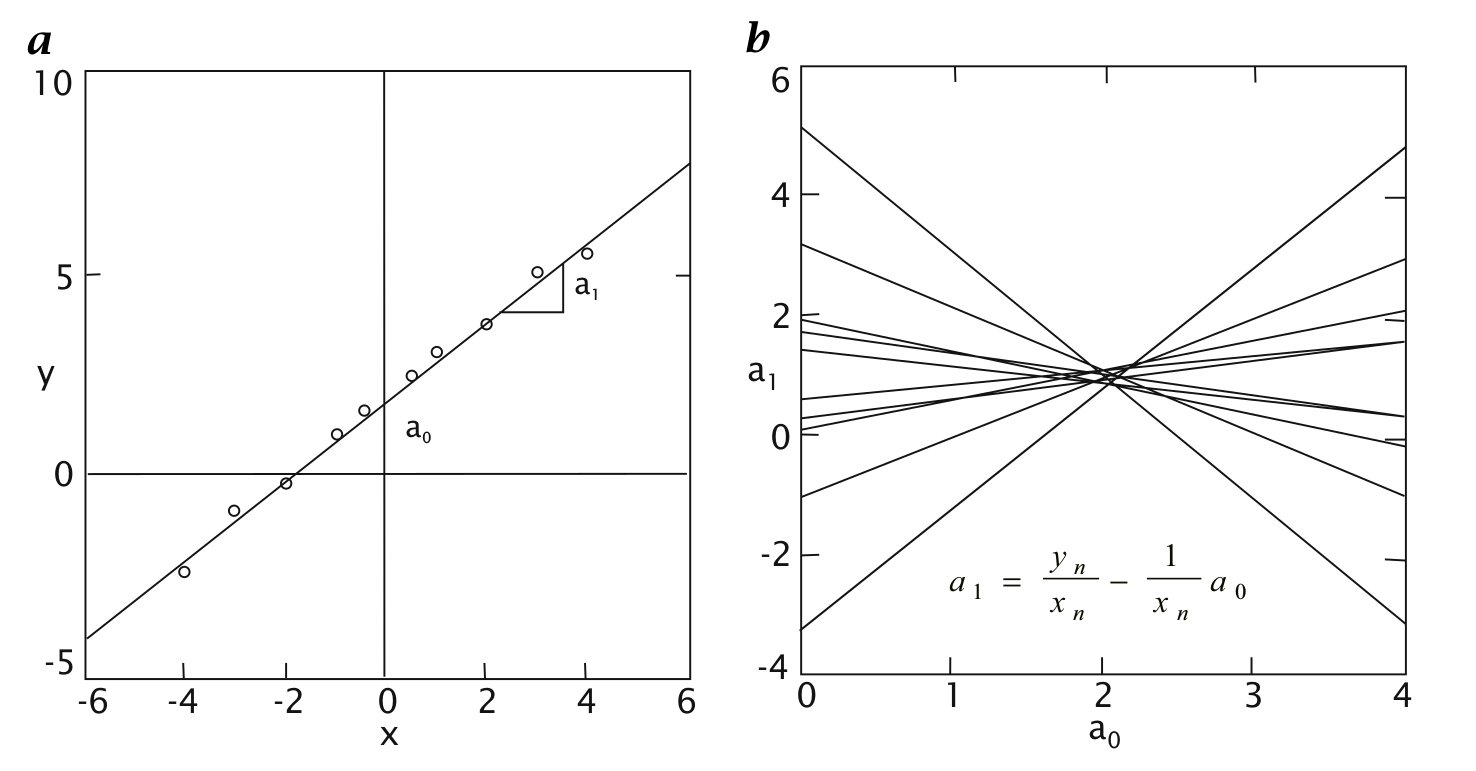
\includegraphics[width=0.9\textwidth]{grundlagen_hough.png}
  \caption{Houghtransformation von Geraden: Punkte aus dem Datenraum (\textbf{a}) werden auf den Modellraum (\textbf{b}) abgebildet.}
%  \label{fig:grundlagen_hough}
\end{figure} 

Praktischerweide wird als Modell für die Gerade eigentlich die hesse'sche Normalform (Steigungswinkel und Abstand zum Koordinatenursprung als Parameter) eingesetzt, da die Beschreibung in~\ref{eq:geradengleichung} den großen Nachteil hat, dass der Parameter \( a_1 \) bei vertikalen Geraden ins Unendliche läuft. 

\subsection{vereinfachte Hough-Transformation}
% Hier fehlt der Verweis auf BA_Marcel_Unger
Wir haben in unserer Arbeit in Anlehnung an \autocite{} eine sehr vereinfachte Form der Hough-Transformation zur Anwendung gebracht, welche nur zu einer alternativen Initialisierung eines Startpunktes zum Einsatz kommt. Die angewendete Methode sucht ausschließlich nach vertikalen Linien im Bild. Dazu wird ein Histogramm über die Spaltensummen der Pixelmatrix gebildet. Die Lage der Maxima über einem bestimmten Threshold-Wert geben dann Auskunft über die Position einer näherungsweise vertikal erkannten Gerade.